%!TEX root = ../main.tex

\chapter{Datenmodell}
\label{ch:datamodel}

\todo{add DATAMODEL, ER diagramm}


\section{ER-Diagramm}

AUf Grund einiger Änderungen im Datenmodell, wurde das ER-Diagramm angepasst.
Einer der Gründe ist zum Beispiel die Einführung von den Öffnungszeiten.

In \ref{fig:er-diagramm} finden sie das alte ER-Diagramm aus dem Entwurfsheft und in \ref{fig:er-diagramm_new} das neue ER-Diagramm.

Zum besseren Verständnis ist in \ref{fig:er-diagramm_legend} eine Legende für das ER-Diagramm.

\begin{figure}[ht]
    \centering
    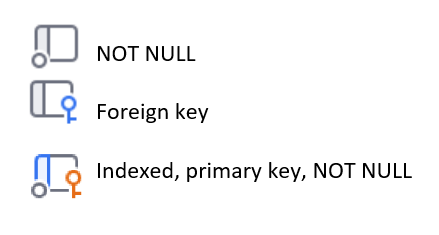
\includegraphics[width=\textwidth]{figures/ERLegend}
    \caption{Legende: ER-Diagramm}
    \label{fig:er-diagramm_legend}
\end{figure}

\begin{figure}[ht]
    \centering
    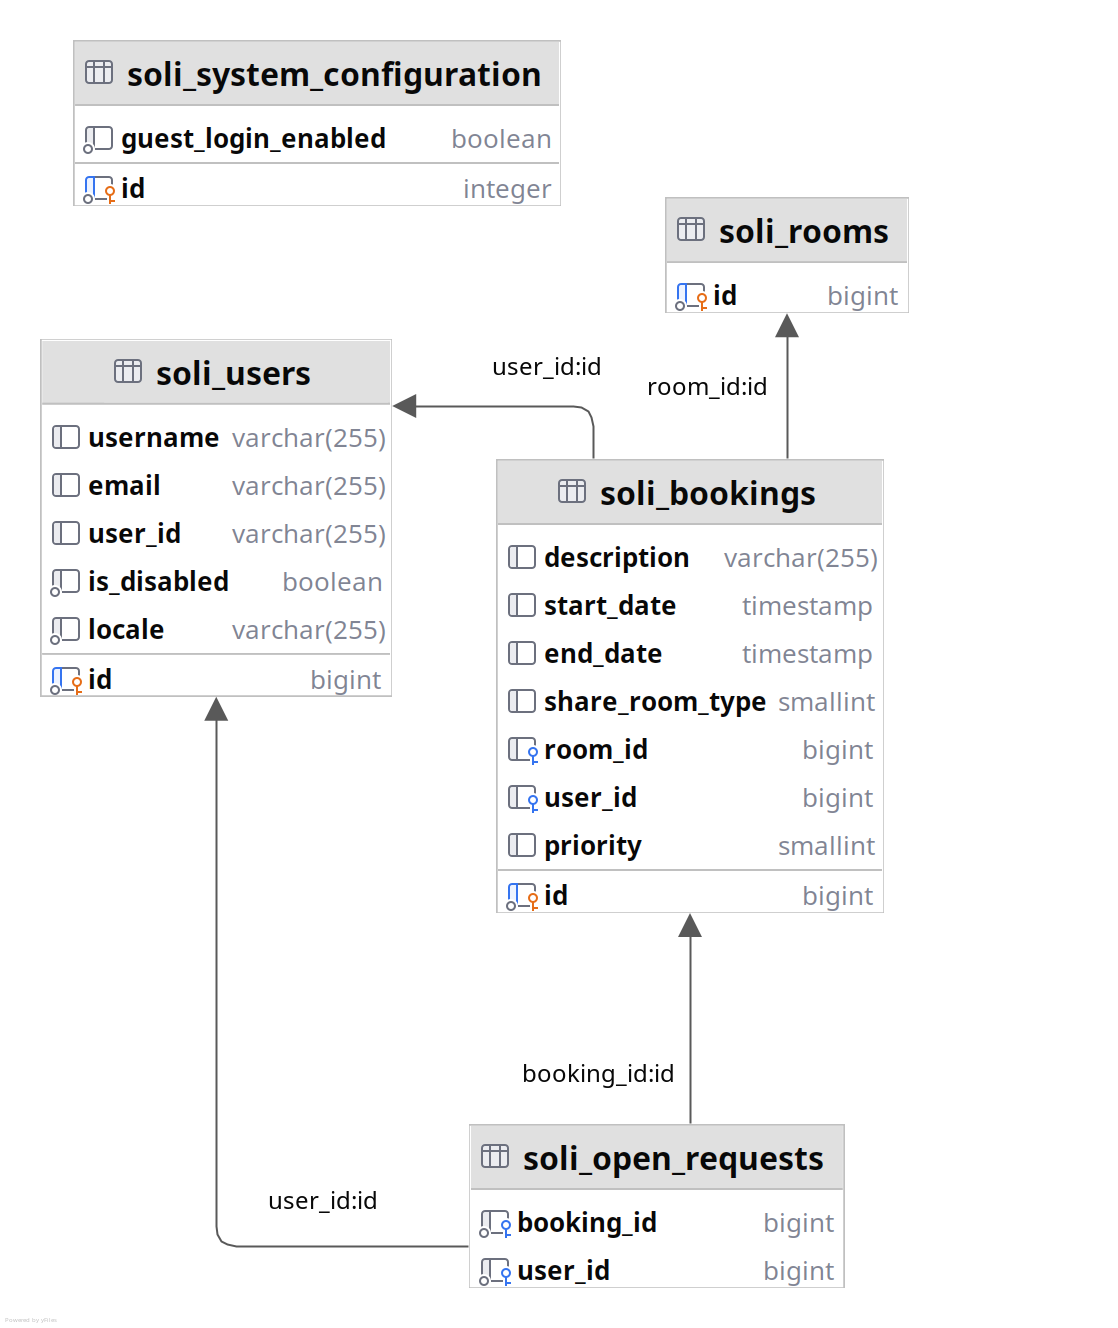
\includegraphics[width=\textwidth]{figures/database}
    \caption{ER-Diagramm}
    \label{fig:er-diagramm}
\end{figure}

\begin{figure}[ht]
    \centering
    
\includegraphics[width=\textwidth]{figures/impl-views/placeholder} % TODO add new ER-Diagramm (in lightmode pls)
    \caption{Neues ER-Diagramm}
    \label{fig:er-diagramm_new}
\end{figure}